\documentclass[11pt, letterpaper]{article}
\usepackage[letterpaper, margin=1in]{geometry}
\usepackage{graphicx}
\usepackage[dvipsnames]{xcolor}
\definecolor{linkbordergray}{rgb}{0.8,0.8,0.8}
\usepackage[linkbordercolor=linkbordergray]{hyperref}
\graphicspath{{images/}}

\newcommand{\overbar}[1]{\mkern 1.5mu\overline{\mkern-1.5mu#1\mkern-1.5mu}\mkern 1.5mu}

\title{AM9511 Interface for the 6502}
\author{Carl Harris}
\date{December 2024}
\begin{document}
\maketitle
\noindent 
The AMD AM9511 Arithmetic Processing Unit, first produced in the late 1970s, 
provides high performance fixed or floating point arithmetic as well as
common transcendental functions. It provides an excellent enhancement to any 
retro-computer that will be used to perform fixed-point or floating-point 
mathematical operations. At present, these parts are obtainable from various 
suppliers as new-old stock or used stock.

This article describes an interface allowing the AM9511A to be directly 
connected to the bus of the 6502 microprocessor. It is adapted from the work 
of Kissel or Currie\footnote{Kissel, R and Currie, J: 
\emph{Hardware Math for the 6502 Microprocessor}; July 1985; 
NASA TM-86517} in which they developed an experiment using a MOS 6502 
microprocessor to control four AM9511A floating-point arithmetic units. It
also includes elements of Hart’s MICROCRUNCH\footnote{Hart, J: 
\emph{MICROCRUNCH: An Ultra-Fast Arithmetic Computing System (part 1)}; 
August 1981; MICRO - the 6502/6809 Journal} which used the AM9511A 
(Intel 8231A) interfaced with a (Rockwell) 6502.

\section{Bus Interface Design}
The AM9511 uses an asynchronous interface design -- its timing is not derived 
from the clock of the host microprocessor. This allows the AM9511A to be 
clocked at 4 MHz while, in the case of the original 6502, the system clock 
is only 1 MHz. A disadvantage of this approach is that the interface has 
some strict timing requirements to ensure that the actions of the AM9511 
or the microprocessor are effectively coordinated, despite the lack of a 
shared clock.

The bus signal timing requirements of the AM9511 are generally easy to 
satisfy using microprocessors such as the 8080, 8085, or Z80, all of which
are designed to use multiple clock cycles for each machine cycle. In such 
systems, the bus control signals for addressing or read/write control are 
changed over the course of multiple clock cycles, with addressing (chip 
selection) happening first, followed by changes to read or write signals 
in later cycles. At the end of a cycle, the read and write signals change
first, before changes to the address lines.

In the 6502, after the falling edge of the clock, addressing and read/write 
selection are stabilized at effectively the same time. At the next rising 
clock edge, a read or write operation occurs, ending at the subsequent 
falling edge at which time the addressing and read/write selection signals 
are subject to change again.

The AM9511 requires the address input ($C/\overbar{D}$) to be stable before 
the chip select ($\overbar{CS}$) and read ($\overbar{RD}$) or write 
($\overbar{WR}$) signals are asserted. The minimum delay between the fall of 
$\overbar{CS}$ and the fall of either $\overbar{RD}$ or $\overbar{WR}$ is 
given as zero, which simply means that $\overbar{RD}$ or $\overbar{WR}$ 
cannot precede $\overbar{CS}$. This is generally easy to satisfy in a 
6502-based system.

The first complication involves write operations. The AM9511 requires a 
minimum positive delay between the rise of the $\overbar{WR}$ signal (at 
he end of a write operation) and the rise of the $\overbar{CS}$ signal. 
Depending on the specific AM9511 part, this delay requirement could be as 
high as 60 ns. Obviously, this requirement precludes direct use of the 
$R/\overbar{W}$ signal as the input to $\overbar{WR}$, since $R/\overbar{W}$ 
changes state coincident with the address lines soon after the falling edge 
of the $PHI2$ clock.

As suggested by Hart, the solution here uses a monostable multivibrator to 
effectively control the length of the low pulse on the $\overbar{WR}$ signal. 
As shown in Figure \ref{fig:schematic}, the circuit uses a 74HC123 
monostable multivibrator. This part is used because it is easy to get a fixed 
delay in the monostable pulse, without regard to the length of the trigger 
pulse. The combination of a 68 pF capacitor and a 2.4 K\textohm\  resistor 
provides an output pulse of approximately 75 ns which is sufficient to meet 
the delay requirement for any AM9511 part, while still being significantly 
shorter than one half of the $PHI2$ clock period.

\begin{figure}[h]
\centering
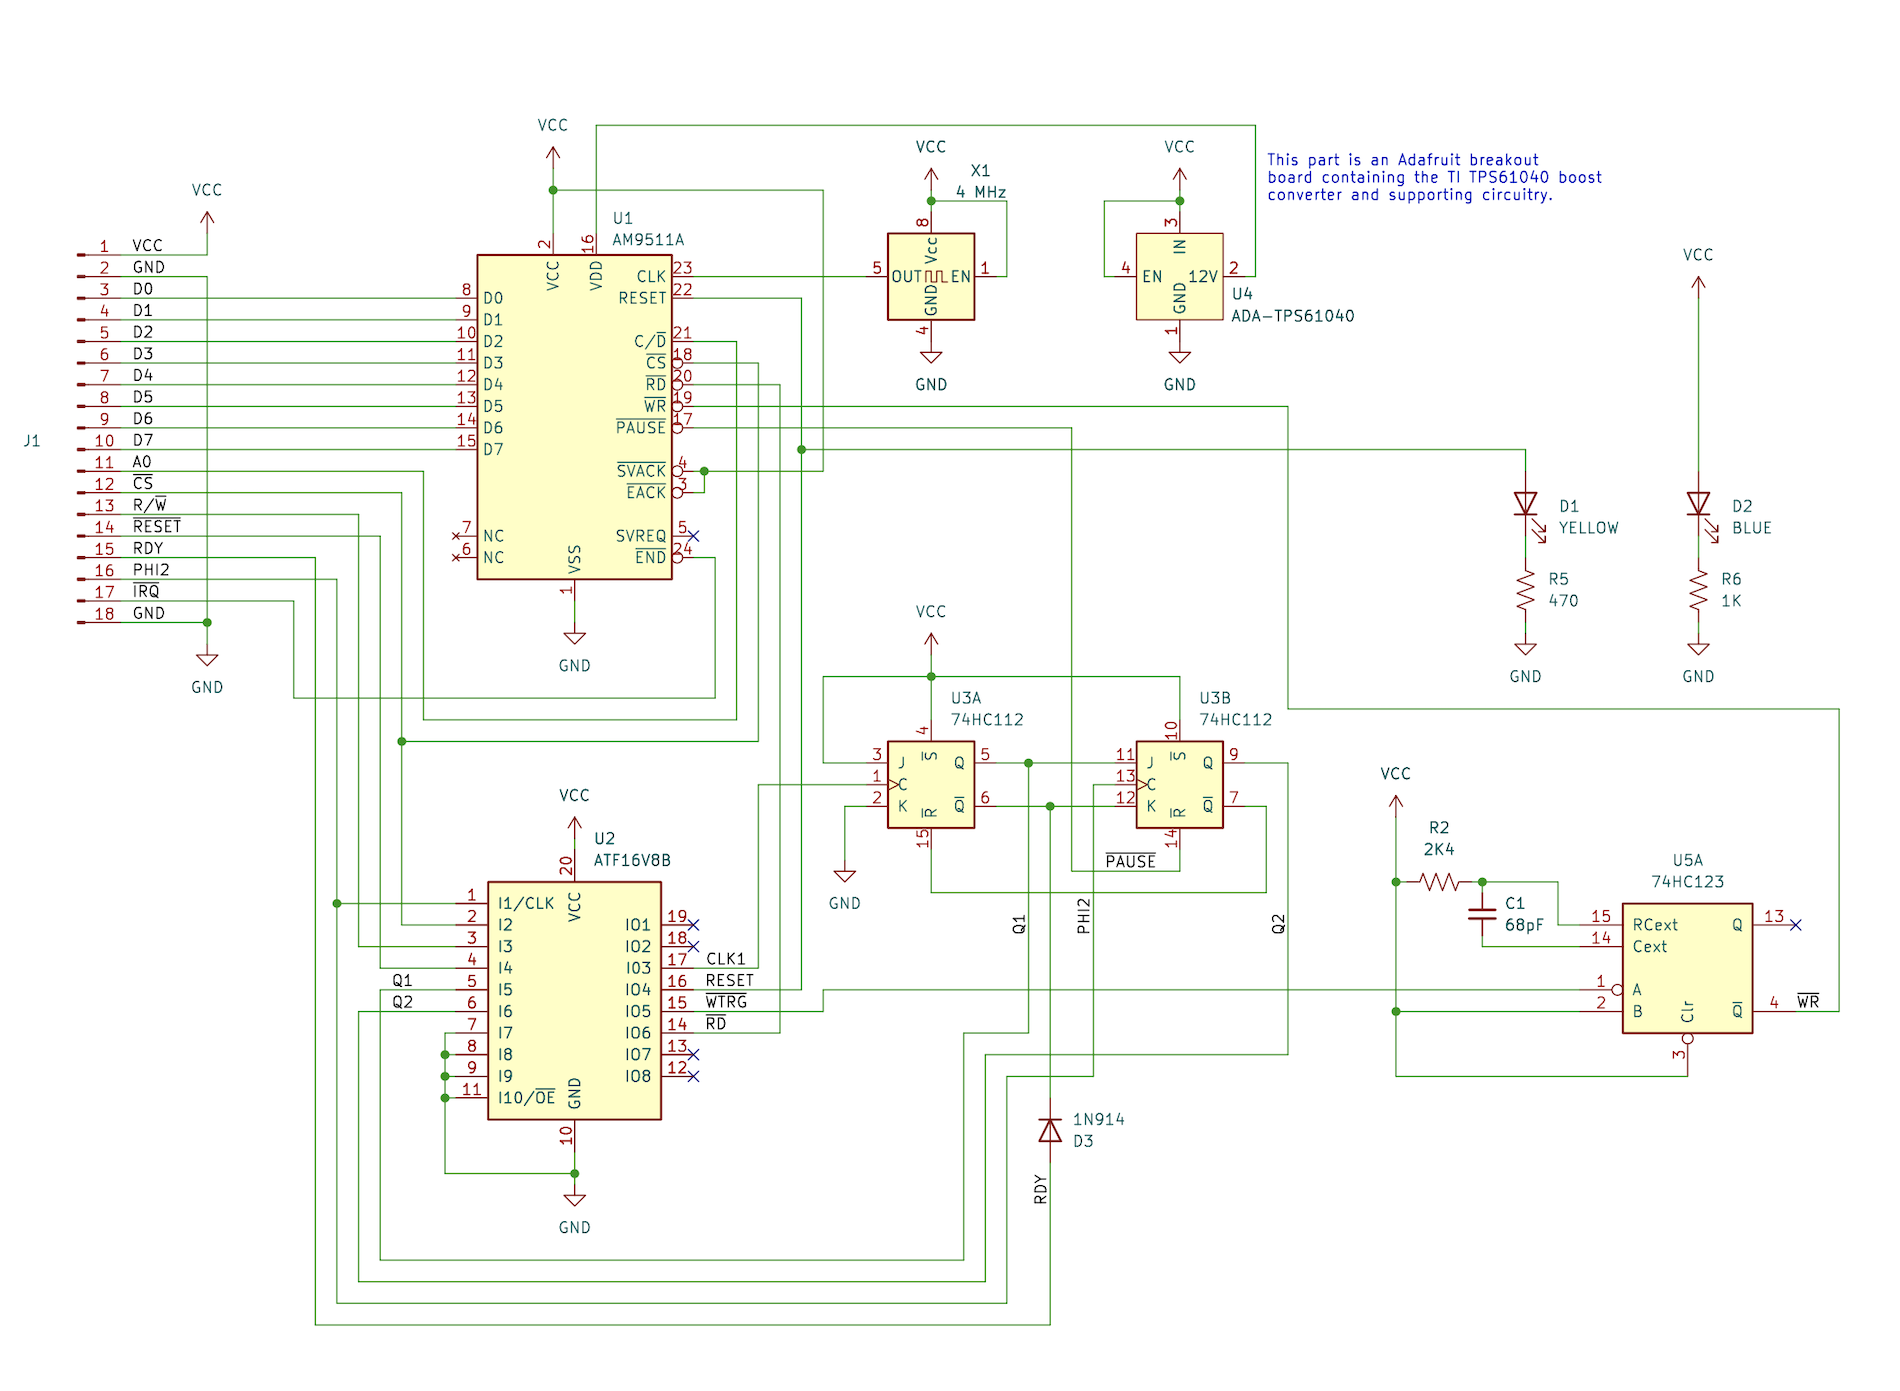
\includegraphics[width=1\textwidth]{schematic.png}
\caption{Circuit Schematic}
\label{fig:schematic}
\end{figure}

In a read operation, it is assumed that the microprocessor will 
set $C/\overbar{D}$, then assert $\overbar{CS}$ and $\overbar{RD}$.
The AM9511 then asserts its $\overbar{PAUSE}$ output, which remains 
low until the requested data is available on lines $D[0..7]$. When 
the data is available, the AM9511 releases $\overbar{PAUSE}$ and lines
$D[0..7]$ remain stable until $\overbar{RD}$, $\overbar{CS}$, 
or $C/\overbar{D}$ changes. The minimum delay between the rise of 
$\overbar{RD}$ and the rise of $\overbar{CS}$ is given as zero -- 
in particular, this implies that $\overbar{RD}$ cannot rise \emph{after}
 $\overbar{CS}$.

The intent of the $\overbar{PAUSE}$ signal in a read operation is to 
force the microprocessor to wait until data requested from the AM9511 
becomes available on the bus. The 6502 has an active high $RDY$ input 
that inserts wait states for this purpose. A complication arises from 
the fact that the 6502 observes the state of this input on the rising 
edge of the $PHI2$ clock - i.e. at the instant at which the 6502 would 
perform the read operation, if $RDY$ is low it will instead wait until 
the next rising edge of the clock at which time it will again observe 
the state of RDY. After $\overbar{RD}$ is asserted, the AM9511 may 
require as much as 150 ns before $\overbar{PAUSE}$ is asserted. 
Depending on the $PHI2$ clock frequency and the time that it takes for 
the address and $R/\overbar{W}$ lines to settle, this could occur 
\emph{after} the rising edge of the clock cycle in which the read 
operation was initiated.

Asserting the AM9511’s $\overbar{RD}$ after the falling edge of the 
clock is further complicated by the fact that the 6502 can arbitrarily 
change the state of the address lines and $R/\overbar{W}$ immediately 
after the falling edge of the $PHI2$ clock. We must be careful to avoid
asserting $\overbar{RD}$ spuriously while the 6502’s signals are 
settling -- doing so could inadvertently trigger a read operation, 
unexpectedly disrupting the state of the AM9511’s stack.

To solve both of these complications with read operations, the solution
here is basically the same as that used by Kissel and Currie -- a pair 
of JK flip-flops that latch $RDY$ in the low state at the beginning of an
operation, and reset it to the high state after the $\overbar{PAUSE}$ 
signal rises. The state of these flip-flops is also used as an enable for 
the $\overbar{RD}$ signal.

This circuit uses a programmable logic device (ATF16V8) to implement the 
necessary combinatorial logic. This could also be done with discrete 7400 
series logic circuits, but the ATF16V8 is readily available and easily 
programmed using open-source tools Galette\footnote{\emph{Galette: A 
GAL assembler, largely galasm-compatible and written in Rust}; \\
\url{https://github.com/simon-frankau/galette}} 
and Minipro\footnote{\emph{Minipro: An open source program for controlling 
the MiniPRO TL866xx series of chip programmers}; \\
\url{https://gitlab.com/DavidGriffith/minipro}}. 
Figure 
\ref{fig:pld-logic} shows the logic programmed into the PLD.

\begin{figure}[h]
\centering
\includegraphics[width=0.8\textwidth]{pld-logic.png}
\caption{Combinatorial Logic}
\label{fig:pld-logic}
\end{figure}

With this logic, the $\overbar{WTRG}$ signal is asserted at the rising
edge of $PHI2$ if the $\overbar{CS}$ signal is asserted and $R/\overbar{W}$ 
is low. This output provides the trigger input for the 74HC123 used to 
produce the $\overbar{WR}$ pulse for the AM9511.

The $Q1$ and $Q2$ inputs to this logic are the corresponding outputs of 
the JK flip-flops. These are logically OR'ed as an enable signal to prevent 
$\overbar{RD}$ from being asserted spuriously. The CLK1 output connects to 
the clock input of the first flip-flop. Since the 74HC112 has a negative 
edge trigger, the falling edge of this signal (when $\overbar{CS}$ is 
asserted and R/$\overbar{W}$ is high) clocks a logic one into the first 
flip-flop, and simultaneously drives the $\overbar{RD}$ signal low.

The $\overbar{Q1}$ output of the first flip-flop is connected to the 6502’s 
$RDY$ input, so a logic one in this flip-flop signals to the 6502 that it 
should wait at the next rising edge of $PHI2$. The clock input of the second 
flip-flop is tied to $PHI2$, so at the next falling edge of $PHI2$ for which 
the AM9511’s $\overbar{PAUSE}$ output is not asserted, the second flip-flop 
will clock in a logic one. Output $Q2$ will be high, so $\overbar{RD}$ will 
continue to be asserted even though output $\overbar{Q2}$ will reset the 
first flip-flop, signaling to the 6502 that it can continue. The next rising 
edge of the $PHI2$ will complete the read operation, and the subsequent 
falling edge of $PHI2$ will cause the second flip-flop to clock in a logic 
zero (because $J2$ is low while $K2$ is high).

The only other significant elements of the circuit are the 4 MHz clock 
oscillator and a boost converter.

The AM9511A-4DC can run at 4 MHz. Other parts, such as the AM9511A-1DC require 
a clock speed no greater than 3 MHz. I decided to use a dedicated on-board
clock oscillator mostly as a matter of convenience. Of course, the AM9511 could
be clocked by the system clock (with an appropriate divider circuit if necessary).

The AM9511 requires a +12V DC bias input. I choose to use a boost converter
since the current requirement is quite small, and doing so avoids the complication
of a having multiple DC supplies at different voltages. The boost converter depicted
in the schematic is a breakout board made by Adafruit. However, any +5 VDC to +12 VDC 
boost converter should be fine -- only about 100 mA current is needed at +12 VDC. 

\section{Other Considerations}

The interface described herein does not provide a mechanism to wait after a write
operation. This means that even though the AM9511 asserts the $\overbar{PAUSE}$ 
signal while executing a requested operation, the 6502 will not wait until the 
requested operation is completed. This allows the programmer to decide how best 
to use the time during which an operation is executing. One simple approach is 
to simply poll the BUSY flag in the AM9511's status register in a loop
to determine when a requested operation has completed execution. 

Alternatively, the hardware could make use of the $\overbar{END}$ signal (or 
$SVREQ$ signal) as an interrupt source to allow other work to be completed 
concurrently while the AM9511 is executing operations. The module described 
here can connect $\overbar{END}$ to the 6502's $\overbar{IRQ}$ input if desired.
The $\overbar{END}$ signal is an open-drain output, allowing it to be easily
incorporated into a design that uses a wired-OR configuration for multiple
devices connected to the 6502's $\overbar{IRQ}$ input.

Furht and Lee\footnote{Furht, B and Lee, P: \emph{An Efficient Software Driver 
for AM9511 Arithmetic Processor Implementation}; June 1984; IEEE Micro, Volume 4
Issue 3} describe an interrupt-driven approach for the 8085 microprocessor that
could be adapted for the 6502. Using such a design, is it possible to enqueue a
sequence of interdependent operations in main memory, pushing operands and
operations onto the AM9511's stack as soon as it is able to accommodate them.


\pagebreak
\section{Observed Timing}

The following oscilloscope plots show key aspects of the interface timing as 
observed using a WDC 65C02 clocked at 1.8432 MHz and the AM9511A clocked at 
4 MHz.

\subsection{Write Operation}

Figure \ref{fig:write-timing} shows the timing for a write operation. A 
write operation targeting the dataregister versus the command register differs 
only in the value of the $C/\overbar{D}$ signal (shown here as $A0$) -- it is 
high here signifying a write to the command register. Note that the 
$\overbar{WR}$ pulse falls soon after the rising edge of $PHI2$ but rises 
approximately 75 ns before either $\overbar{CS}$ or $A0$ changes state. This 
satisfies what amounts to the most critical timing constraint of the AM9511.

\begin{figure}[h]
\centering
\includegraphics[width=1\textwidth]{write-ctrl.png}
\caption{Write Operation Timing}
\label{fig:write-timing}
\end{figure}

\pagebreak
\subsection{Read Operation}

Figure \ref{fig:read-timing} shows the timing of a read operation. The 
$C/\overbar{D}$ input is not shown here since the scope has but four analog 
channels. However, this signal follows the same timing as the $\overbar{CS}$ 
signal. Here we can see that when $\overbar{CS}$ is asserted, the 
$\overbar{RD}$ signal goes low after a short delay.  In response to the read 
request, the AM9511 pulls $\overbar{PAUSE}$ low indicating that it is busy 
accessing the requested data. After the $\overbar{PAUSE}$ signal rises, at 
the next rising edge of $PHI2$, the read operation is completed. By counting 
the rising edges between the transitions of $\overbar{CS}$ from high to low 
and back to high again, we can see that a total of four cycles were needed to 
complete the read operation.

\begin{figure}[h]
\centering
\includegraphics[width=1\textwidth]{read-pause.png}
\caption{Read Operation Timing}
\label{fig:read-timing}
\end{figure}

\pagebreak
\subsection{Timing of the RDY Signal}

In order to see the timing associated with the 6502’s $RDY$ signal, in Figure 
\ref{fig:read-ready}, $\overbar{RD}$ has been replaced with $RDY$. As shown
in Figure \ref{fig:read-timing}, $\overbar{RD}$ has essentially the same timing 
as $\overbar{CS}$ so they can be considered equivalent for our purposes here.

Note that $RDY$ falls at virtually the same instant as $\overbar{CS}$ as the 
first flip-flop is clocked to logic one by $\overbar{CS}$ whenever the 6502’s 
$R/\overbar{W}$ signal is high. Subsequently, the $\overbar{PAUSE}$ signal 
goes low, preventing the second flip-flop from clocking in logic one on 
subsequent falling edges of PHI2. Before the third falling edge of $PHI2$, 
$\overbar{PAUSE}$ rises, and subsequently the second flip-flop clocks in a 
logic one, causing the first flip-flop to reset and asserting $RDY$. This 
allows the read operation to be completed at the next rising edge of $PHI2$.

\begin{figure}[h]
\centering
\includegraphics[width=1\textwidth]{read-ready-pause.png}
\caption{RDY Signal Timing}
\label{fig:read-ready}
\end{figure}


\end{document}